\chapter{Teorema de Pitágoras}
\begin{list}{\textbf{Questão \arabic{quest}.}}{\usecounter{quest}}
%define a margem da lista.	
%\setlength{\labelwidth}{-2mm} \setlength{\parsep}{0mm}
%\setlength{\topsep}{0mm} \setlength{\leftmargin}{-2mm}
\renewcommand{\labelenumi}{(\alph{enumi})}

\item Aplicando o teorema de Pitágoras, determine a medida x indicada em cada um dos triângulos retângulos.
	\begin{multicols}{2}
	\begin{enumerate}
		\item 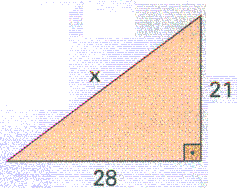
\includegraphics[scale=0.5]{figuras/fig68.png}
		\item 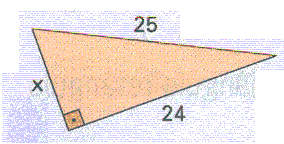
\includegraphics[scale=0.5]{figuras/fig69.png}
		\item 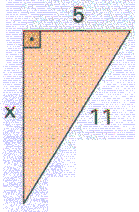
\includegraphics[scale=0.5]{figuras/fig70.png}
		\item 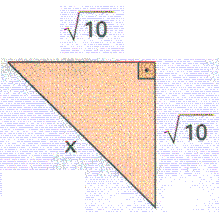
\includegraphics[scale=0.5]{figuras/fig71.png}
		\item 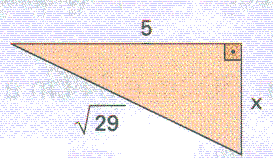
\includegraphics[scale=0.5]{figuras/fig72.png}
		\item 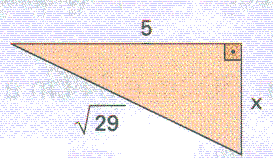
\includegraphics[scale=0.5]{figuras/fig72.png}
		\item 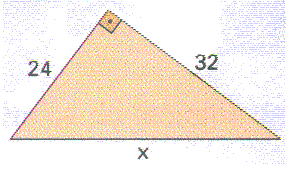
\includegraphics[scale=0.5]{figuras/fig73.png}		
	\end{enumerate}
	\end{multicols}
	
	\item Os lados de um triângulo ABC medem 10cm, 24cm e 26cm. Você pode afirmar que esse triângulo é retângulo?


	\item Em um triângulo retângulo, a hipotenusa mede 14cm e um dos catetos mede $5\sqrt{3}$ cm. Determine a medida do outro cateto.

	\item As medidas dos catetos de um triângulo retângulo medem $(2+\sqrt{5})$ cm e $(-2+\sqrt{5})$ cm. Determine a medida da hipotenusa.

	\item Um terreno triangular tem frentes de 12m e 16m em duas ruas que formam um ângulo de 90º. Quanto mede o terceiro lado desse terreno?

	\item O portão de entrada de uma casa tem 4m de comprimento e 3m de altura. Que comprimento teria uma trave de madeira que se estendesse do ponto A até o ponto C?
\begin{center}
		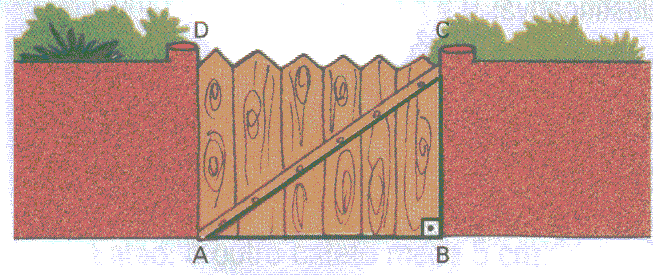
\includegraphics[scale=0.5]{figuras/fig74.png}

	\end{center}	
	\item Dois navios partem de um mesmo ponto, no mesmo instante, e viajam com velocidades constante em direções que formam um ângulo reto. Depois de uma hora de viagem, a distância entre os dois navios é 13 milhas. Se um deles é 7 milhas por hora mais rápido que o outro, determine a velocidade de cada navio.
\begin{center}
		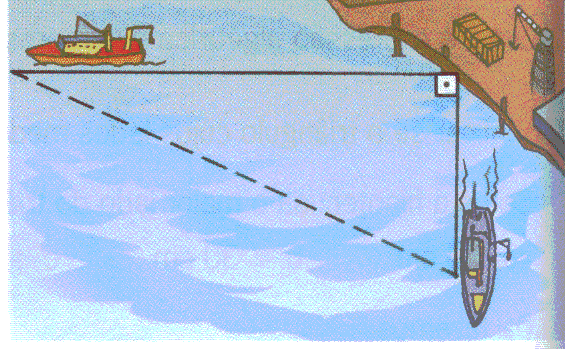
\includegraphics[scale=0.5]{figuras/fig75.png}

	\end{center}	
	\item Durante um incêndio num edifício de apartamentos, os bombeiros utilizaram uma escada Magirus de 10 m para atingir a janela do apartamento sinistrado. A escada estava colocada a 1m do chão, sobre um caminhão que se encontrava afastado 6m do edifício. Qual é a altura do apartamento sinistrado em relação ao chão?
\begin{center}
		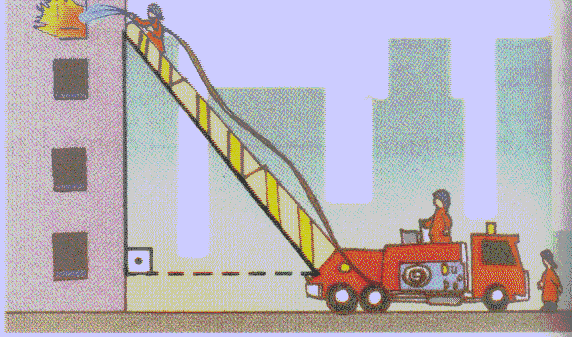
\includegraphics[scale=0.5]{figuras/fig76.png}

	\end{center}	
	\item Quantos metros de fio são necessários para "puxar luz" de um poste de 6m de altura até a caixa de luz que está ao lado da casa e a 8m da base do poste?
\begin{center}
		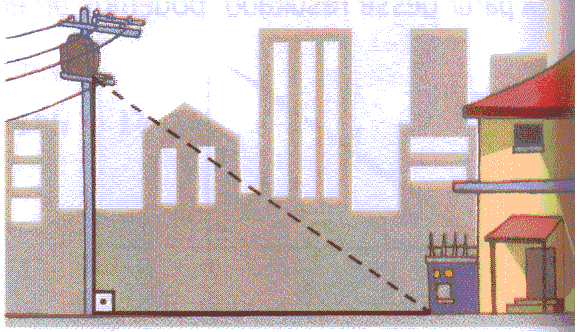
\includegraphics[scale=0.5]{figuras/fig77.png}

	\end{center}	
	\item Na figura, o triângulo BCD é equilátero.
\begin{center}
	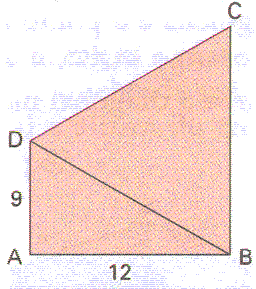
\includegraphics[scale=0.5]{figuras/fig78.png}

\end{center}
Determine:
	\begin{enumerate}
	\item o perímetro do triângulo BCD.
	\item o perímetro do quadrilátero ABCD
	\end{enumerate}
	\item Na figura tem-se que $\overline{AB} \cong \overline{BC}$ e F é o ponto médio do lado $\overline{BE}$ do retângulo BCDE. 
	Determine 
\begin{center}
		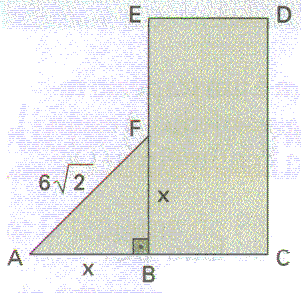
\includegraphics[scale=0.5]{figuras/fig79.png}	

	\end{center}	\begin{enumerate}
	\item a medida x indicada na figura.
	\item a área do retângulo BCDE.		
	\end{enumerate}
	
\end{list}